\documentclass{article}

\usepackage{graphicx}
\usepackage{tikz}
\usepackage{tikzsymbols}
\usetikzlibrary{calc,patterns,shapes.geometric}
\pagestyle{empty}
\usepackage[margin=0pt]{geometry}
\geometry{papersize={14in,12in}}

\def\centerarc[#1](#2)(#3:#4:#5){\draw[#1] ($(#2)+({#5*cos(#3)},{#5*sin(#3)})$) arc (#3:#4:#5);}

\begin{document}
	\begin{figure}
		\centering
		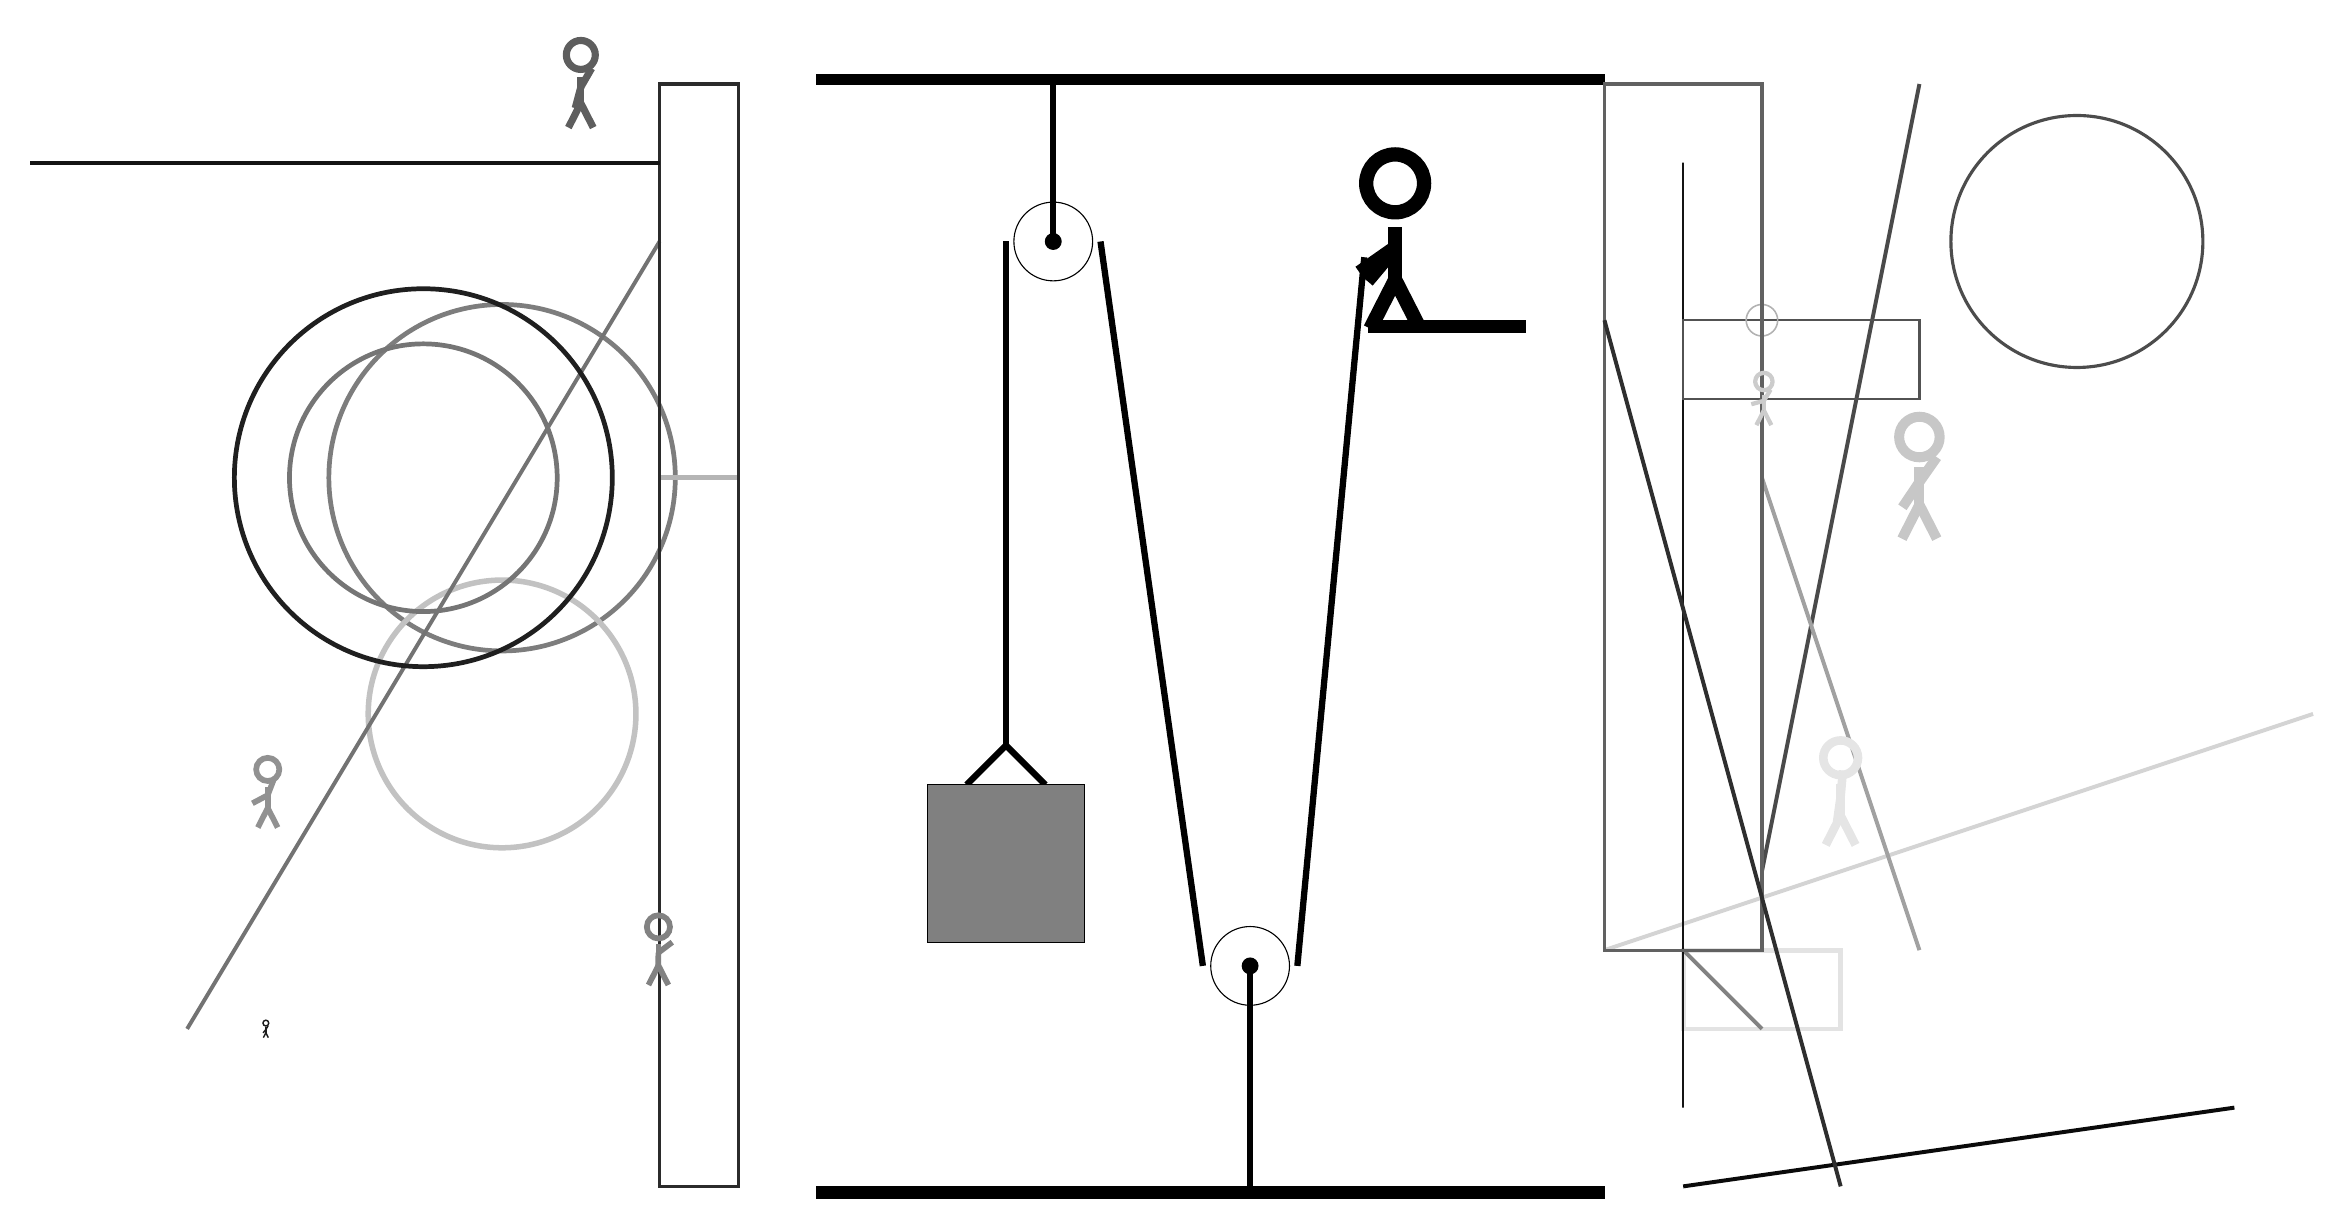
\begin{tikzpicture}
			%%%%% START %%%%%
			
			\draw[fill=black] (-2, 14) rectangle (8, 14.125);
			
			\draw (3.5, 2.8) circle (0.5);
			\draw[fill=black] (3.5, 2.8) circle (0.1);
			\draw[line width=0.8mm] (3.5, 2.8) -- (3.5, 0);
			
			\draw (1, 12) circle (0.5);
			\draw[fill=black] (1, 12) circle (0.1);
			\draw[line width=0.8mm] (1, 14) -- (1, 12);
			
			\draw[line width=0.8mm](-0.1, 5.1) --  (0.4, 5.6) -- (0.9, 5.1);
			\draw[fill=black!50] (-0.6, 5.1) rectangle (1.4, 3.1);
			
			\draw[line width=0.8mm](0.4, 12) -- (0.4, 5.6);
			\centerarc[line width=0.8mm](1, 12)(180:0:0.6)
			\draw[line width=0.8mm](1.6, 12) -- (2.9, 2.8);
			\centerarc[line width=0.8mm](3.5, 2.8)(180:360:0.6)
			\draw[line width=0.8mm](4.1, 2.8) -- (4.95, 11.8);
			
			\draw[line width=0.5mm, color=black!17](8, 3) -- (17, 6);
			
			\draw[line width=0.6mm, color=black!11] (9, 3) rectangle (11, 2);
			\draw[line width=0.5mm, color=black!49](10, 2) -- (9, 3);
			\draw[line width=0.5mm, color=black!96](9, 0) -- (16, 1);
			
			\draw [line width=0.6mm, color=black!51](-6, 9) circle (2.2);
			
			\draw [line width=0.7mm, color=black!24](-6, 6) circle (1.7);
			\draw [line width=0.4mm, color=black!70](14, 12) circle (1.6);
			
			\draw[line width=0.5mm, color=black!55](-4, 12) -- (-10, 2);
			\draw[line width=0.6mm, color=black!29] (-4, 9) rectangle (-3, 9);
			
			\node[line width=0.6mm, color=black!43] at (-9, 5) {\Strichmaxerl[4][28][69]};
			\draw[line width=0.4mm, color=black!83] (-4, 14) rectangle (-3, 0);
			\draw[line width=0.2mm, color=black!92] (9, 1) rectangle (9, 13);
			\draw[line width=0.5mm, color=black!71](10, 4) -- (12, 14);
			
			\draw[line width=0.3mm, color=black!68] (9, 11) rectangle (12, 10);
			\draw[line width=0.5mm, color=black!92](-4, 13) -- (-12, 13);
			\draw[line width=0.5mm, color=black!37](12, 3) -- (10, 9);
			\draw [line width=0.6mm, color=black!54](-7, 9) circle (1.7);
			
			\node[line width=0.6mm, color=black!22] at (12, 9) {\Strichmaxerl[7][56][55]};
			\draw[line width=0.6mm, color=black!68] (-2, 8) rectangle (-2, 8);
			
			\node[line width=0.3mm, color=black!63] at (-5, 14) {\Strichmaxerl[5][75][60]};
			\node[line width=0.5mm, color=black!10] at (11, 5) {\Strichmaxerl[6][82][85]};
			
			\draw [line width=0.2mm, color=black!30](10, 11) circle (0.2);
			
			\node[line width=0.7mm, color=black!89] at (-9, 2) {\Strichmaxerl[1][50][59]};
			\draw[line width=0.4mm, color=black!62] (10, 14) rectangle (8, 3);
			\node[line width=0.5mm, color=black!20] at (10, 10) {\Strichmaxerl[3][15][59]};
			
			\node[line width=0.7mm, color=black!49] at (-4, 3) {\Strichmaxerl[4][89][37]};
			
			\draw [line width=0.6mm, color=black!88](-7, 9) circle (2.4);
			\draw[line width=0.5mm, color=black!82](8, 11) -- (11, 0);
			
			\node at (5.3, 12) {\Strichmaxerl[10][35][-130]};
			\draw[fill=black] (5, 11) rectangle (7, 10.85);
			
			\draw[fill=black] (-2, 0) rectangle (8, -0.15);
			
			%%%%% END %%%%%
		\end{tikzpicture}
	\end{figure}	
\end{document}